\documentclass[1p]{elsarticle_modified}
%\bibliographystyle{elsarticle-num}

%\usepackage[colorlinks]{hyperref}
%\usepackage{abbrmath_seonhwa} %\Abb, \Ascr, \Acal ,\Abf, \Afrak
\usepackage{amsfonts}
\usepackage{amssymb}
\usepackage{amsmath}
\usepackage{amsthm}
\usepackage{scalefnt}
\usepackage{amsbsy}
\usepackage{kotex}
\usepackage{caption}
\usepackage{subfig}
\usepackage{color}
\usepackage{graphicx}
\usepackage{xcolor} %% white, black, red, green, blue, cyan, magenta, yellow
\usepackage{float}
\usepackage{setspace}
\usepackage{hyperref}

\usepackage{tikz}
\usetikzlibrary{arrows}

\usepackage{multirow}
\usepackage{array} % fixed length table
\usepackage{hhline}

%%%%%%%%%%%%%%%%%%%%%
\makeatletter
\renewcommand*\env@matrix[1][\arraystretch]{%
	\edef\arraystretch{#1}%
	\hskip -\arraycolsep
	\let\@ifnextchar\new@ifnextchar
	\array{*\c@MaxMatrixCols c}}
\makeatother %https://tex.stackexchange.com/questions/14071/how-can-i-increase-the-line-spacing-in-a-matrix
%%%%%%%%%%%%%%%

\usepackage[normalem]{ulem}

\newcommand{\msout}[1]{\ifmmode\text{\sout{\ensuremath{#1}}}\else\sout{#1}\fi}
%SOURCE: \msout is \stkout macro in https://tex.stackexchange.com/questions/20609/strikeout-in-math-mode

\newcommand{\cancel}[1]{
	\ifmmode
	{\color{red}\msout{#1}}
	\else
	{\color{red}\sout{#1}}
	\fi
}

\newcommand{\add}[1]{
	{\color{blue}\uwave{#1}}
}

\newcommand{\replace}[2]{
	\ifmmode
	{\color{red}\msout{#1}}{\color{blue}\uwave{#2}}
	\else
	{\color{red}\sout{#1}}{\color{blue}\uwave{#2}}
	\fi
}

\newcommand{\Sol}{\mathcal{S}} %segment
\newcommand{\D}{D} %diagram
\newcommand{\A}{\mathcal{A}} %arc


%%%%%%%%%%%%%%%%%%%%%%%%%%%%%5 test

\def\sl{\operatorname{\textup{SL}}(2,\Cbb)}
\def\psl{\operatorname{\textup{PSL}}(2,\Cbb)}
\def\quan{\mkern 1mu \triangleright \mkern 1mu}

\theoremstyle{definition}
\newtheorem{thm}{Theorem}[section]
\newtheorem{prop}[thm]{Proposition}
\newtheorem{lem}[thm]{Lemma}
\newtheorem{ques}[thm]{Question}
\newtheorem{cor}[thm]{Corollary}
\newtheorem{defn}[thm]{Definition}
\newtheorem{exam}[thm]{Example}
\newtheorem{rmk}[thm]{Remark}
\newtheorem{alg}[thm]{Algorithm}

\newcommand{\I}{\sqrt{-1}}
\begin{document}

%\begin{frontmatter}
%
%\title{Boundary parabolic representations of knots up to 8 crossings}
%
%%% Group authors per affiliation:
%\author{Yunhi Cho} 
%\address{Department of Mathematics, University of Seoul, Seoul, Korea}
%\ead{yhcho@uos.ac.kr}
%
%
%\author{Seonhwa Kim} %\fnref{s_kim}}
%\address{Center for Geometry and Physics, Institute for Basic Science, Pohang, 37673, Korea}
%\ead{ryeona17@ibs.re.kr}
%
%\author{Hyuk Kim}
%\address{Department of Mathematical Sciences, Seoul National University, Seoul 08826, Korea}
%\ead{hyukkim@snu.ac.kr}
%
%\author{Seokbeom Yoon}
%\address{Department of Mathematical Sciences, Seoul National University, Seoul, 08826,  Korea}
%\ead{sbyoon15@snu.ac.kr}
%
%\begin{abstract}
%We find all boundary parabolic representation of knots up to 8 crossings.
%
%\end{abstract}
%\begin{keyword}
%    \MSC[2010] 57M25 
%\end{keyword}
%
%\end{frontmatter}

%\linenumbers
%\tableofcontents
%
\newcommand\colored[1]{\textcolor{white}{\rule[-0.35ex]{0.8em}{1.4ex}}\kern-0.8em\color{red} #1}%
%\newcommand\colored[1]{\textcolor{white}{ #1}\kern-2.17ex	\textcolor{white}{ #1}\kern-1.81ex	\textcolor{white}{ #1}\kern-2.15ex\color{red}#1	}

{\Large $\underline{11n_{133}~(K11n_{133})}$}

\setlength{\tabcolsep}{10pt}
\renewcommand{\arraystretch}{1.6}
\vspace{1cm}\begin{tabular}{m{100pt}>{\centering\arraybackslash}m{274pt}}
\multirow{5}{120pt}{
	\centering
	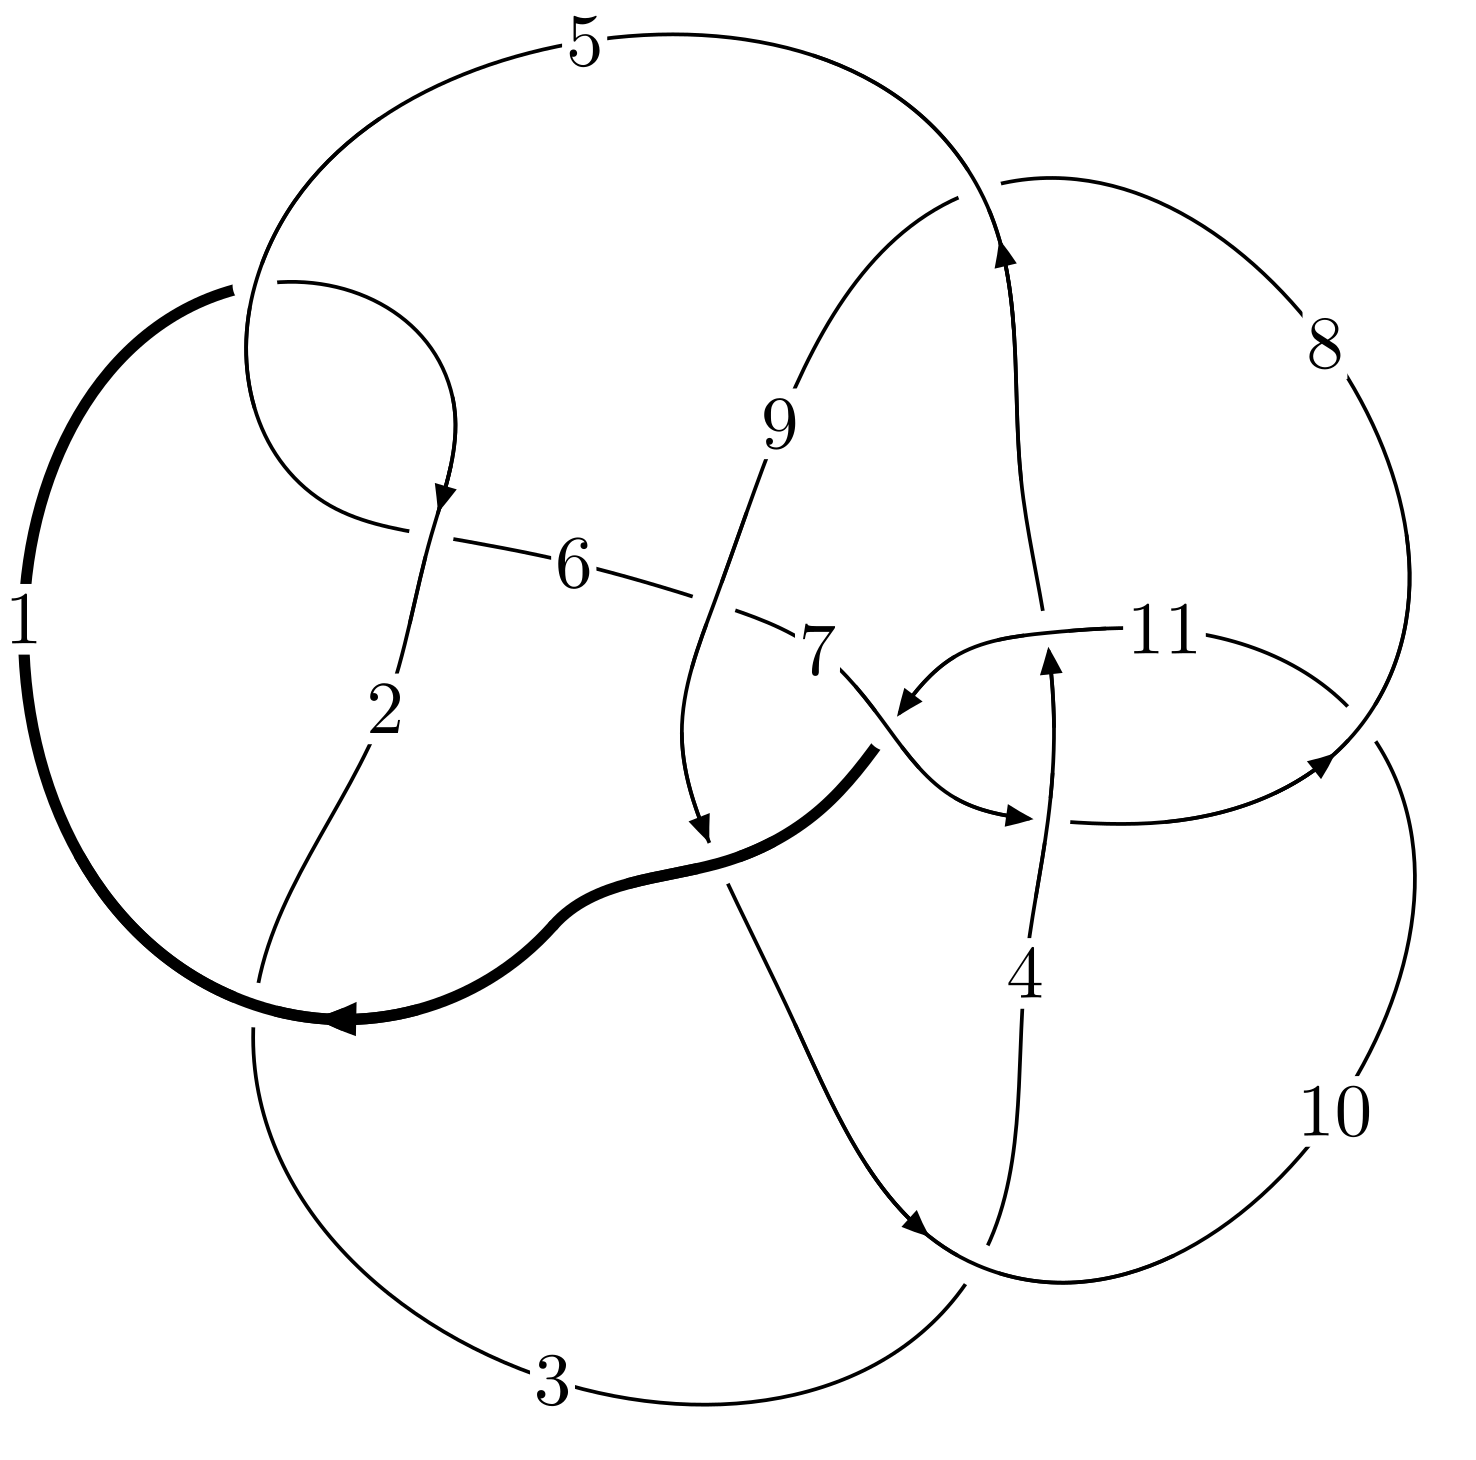
\includegraphics[width=112pt]{../../../GIT/diagram.site/Diagrams/png/749_11n_133.png}\\
\ \ \ A knot diagram\footnotemark}&
\allowdisplaybreaks
\textbf{Linearized knot diagam} \\
\cline{2-2}
 &
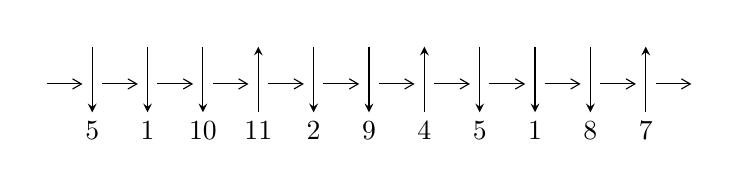
\begin{tikzpicture}[x=20pt, y=17pt]
	% nodes
	\node (C0) at (0, 0) {};
	\node (C1) at (1, 0) {};
	\node (C1U) at (1, +1) {};
	\node (C1D) at (1, -1) {5};

	\node (C2) at (2, 0) {};
	\node (C2U) at (2, +1) {};
	\node (C2D) at (2, -1) {1};

	\node (C3) at (3, 0) {};
	\node (C3U) at (3, +1) {};
	\node (C3D) at (3, -1) {10};

	\node (C4) at (4, 0) {};
	\node (C4U) at (4, +1) {};
	\node (C4D) at (4, -1) {11};

	\node (C5) at (5, 0) {};
	\node (C5U) at (5, +1) {};
	\node (C5D) at (5, -1) {2};

	\node (C6) at (6, 0) {};
	\node (C6U) at (6, +1) {};
	\node (C6D) at (6, -1) {9};

	\node (C7) at (7, 0) {};
	\node (C7U) at (7, +1) {};
	\node (C7D) at (7, -1) {4};

	\node (C8) at (8, 0) {};
	\node (C8U) at (8, +1) {};
	\node (C8D) at (8, -1) {5};

	\node (C9) at (9, 0) {};
	\node (C9U) at (9, +1) {};
	\node (C9D) at (9, -1) {1};

	\node (C10) at (10, 0) {};
	\node (C10U) at (10, +1) {};
	\node (C10D) at (10, -1) {8};

	\node (C11) at (11, 0) {};
	\node (C11U) at (11, +1) {};
	\node (C11D) at (11, -1) {7};
	\node (C12) at (12, 0) {};

	% arrows
	\draw[->,>={angle 60}]
	(C0) edge (C1) (C1) edge (C2) (C2) edge (C3) (C3) edge (C4) (C4) edge (C5) (C5) edge (C6) (C6) edge (C7) (C7) edge (C8) (C8) edge (C9) (C9) edge (C10) (C10) edge (C11) (C11) edge (C12) ;	\draw[->,>=stealth]
	(C1U) edge (C1D) (C2U) edge (C2D) (C3U) edge (C3D) (C4D) edge (C4U) (C5U) edge (C5D) (C6U) edge (C6D) (C7D) edge (C7U) (C8U) edge (C8D) (C9U) edge (C9D) (C10U) edge (C10D) (C11D) edge (C11U) ;
	\end{tikzpicture} \\
\hhline{~~} \\& 
\textbf{Solving Sequence} \\ \cline{2-2} 
 &
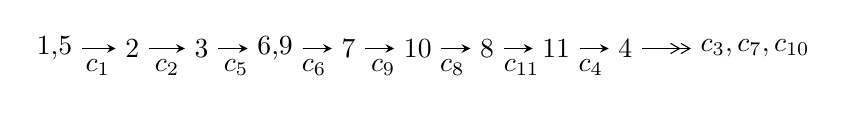
\begin{tikzpicture}[x=25pt, y=7pt]
	% node
	\node (A0) at (-1/8, 0) {1,5};
	\node (A1) at (1, 0) {2};
	\node (A2) at (2, 0) {3};
	\node (A3) at (49/16, 0) {6,9};
	\node (A4) at (33/8, 0) {7};
	\node (A5) at (41/8, 0) {10};
	\node (A6) at (49/8, 0) {8};
	\node (A7) at (57/8, 0) {11};
	\node (A8) at (65/8, 0) {4};
	\node (C1) at (1/2, -1) {$c_{1}$};
	\node (C2) at (3/2, -1) {$c_{2}$};
	\node (C3) at (5/2, -1) {$c_{5}$};
	\node (C4) at (29/8, -1) {$c_{6}$};
	\node (C5) at (37/8, -1) {$c_{9}$};
	\node (C6) at (45/8, -1) {$c_{8}$};
	\node (C7) at (53/8, -1) {$c_{11}$};
	\node (C8) at (61/8, -1) {$c_{4}$};
	\node (A9) at (10, 0) {$c_{3},c_{7},c_{10}$};

	% edge
	\draw[->,>=stealth]	
	(A0) edge (A1) (A1) edge (A2) (A2) edge (A3) (A3) edge (A4) (A4) edge (A5) (A5) edge (A6) (A6) edge (A7) (A7) edge (A8) ;
	\draw[->>,>={angle 60}]	
	(A8) edge (A9);
\end{tikzpicture} \\ 

\end{tabular} \\

\footnotetext{
The image of knot diagram is generated by the software ``\textbf{Draw programme}" developed by Andrew Bartholomew(\url{http://www.layer8.co.uk/maths/draw/index.htm\#Running-draw}), where we modified some parts for our purpose(\url{https://github.com/CATsTAILs/LinksPainter}).
}\phantom \\ \newline 
\centering \textbf{Ideals for irreducible components\footnotemark of $X_{\text{par}}$} 
 
\begin{align*}
I^u_{1}&=\langle 
- u^2+b+u,\;a-1,\;u^5-5 u^4+7 u^3-2 u^2+u-1\rangle \\
I^u_{2}&=\langle 
u^2+b+u,\;a+1,\;u^5+3 u^4+u^3-2 u^2- u+1\rangle \\
I^u_{3}&=\langle 
- u^2 a+b+u,\;a^2- a u+u^2+3 u+3,\;u^3+2 u^2+1\rangle \\
I^u_{4}&=\langle 
- u^5+4 u^4- u^3-8 u^2+4 b+7 u,\;- u^5+3 u^4+3 u^3-11 u^2+4 a-3 u+9,\\
\phantom{I^u_{4}}&\phantom{= \langle  }u^6-4 u^5- u^4+18 u^3-9 u^2-20 u+16\rangle \\
I^u_{5}&=\langle 
- u^2 b+b^2+u^2- u-1,\;a-1,\;u^3+2 u^2+1\rangle \\
I^u_{6}&=\langle 
b+u+1,\;a- u-1,\;u^2+u+1\rangle \\
I^u_{7}&=\langle 
b- a+1,\;a^2- a+1,\;u-1\rangle \\
I^u_{8}&=\langle 
b^2+b+1,\;a+1,\;u-1\rangle \\
\\
\end{align*}
\raggedright * 8 irreducible components of $\dim_{\mathbb{C}}=0$, with total 34 representations.\\
\footnotetext{All coefficients of polynomials are rational numbers. But the coefficients are sometimes approximated in decimal forms when there is not enough margin.}
\newpage
\renewcommand{\arraystretch}{1}
\centering \section*{I. $I^u_{1}= \langle - u^2+b+u,\;a-1,\;u^5-5 u^4+7 u^3-2 u^2+u-1 \rangle$}
\flushleft \textbf{(i) Arc colorings}\\
\begin{tabular}{m{7pt} m{180pt} m{7pt} m{180pt} }
\flushright $a_{1}=$&$\begin{pmatrix}1\\0\end{pmatrix}$ \\
\flushright $a_{5}=$&$\begin{pmatrix}0\\u\end{pmatrix}$ \\
\flushright $a_{2}=$&$\begin{pmatrix}1\\u^2\end{pmatrix}$ \\
\flushright $a_{3}=$&$\begin{pmatrix}- u^2+1\\u^2\end{pmatrix}$ \\
\flushright $a_{6}=$&$\begin{pmatrix}- u\\- u^3+u\end{pmatrix}$ \\
\flushright $a_{9}=$&$\begin{pmatrix}1\\u^2- u\end{pmatrix}$ \\
\flushright $a_{7}=$&$\begin{pmatrix}u^2-2 u\\u^4-3 u^3+u^2+u\end{pmatrix}$ \\
\flushright $a_{10}=$&$\begin{pmatrix}- u^2+u+1\\u^2- u\end{pmatrix}$ \\
\flushright $a_{8}=$&$\begin{pmatrix}1\\- u\end{pmatrix}$ \\
\flushright $a_{11}=$&$\begin{pmatrix}u^3-3 u^2+u+1\\- u^4+2 u^3+u^2- u\end{pmatrix}$ \\
\flushright $a_{4}=$&$\begin{pmatrix}u^3-2 u^2- u+1\\- u^3+2 u^2\end{pmatrix}$\\ \flushright $a_{4}=$&$\begin{pmatrix}u^3-2 u^2- u+1\\- u^3+2 u^2\end{pmatrix}$\\&\end{tabular}
\flushleft \textbf{(ii) Obstruction class $= -1$}\\~\\
\flushleft \textbf{(iii) Cusp Shapes $= 6 u^3-15 u^2-3$}\\~\\
\newpage\renewcommand{\arraystretch}{1}
\flushleft \textbf{(iv) u-Polynomials at the component}\newline \\
\begin{tabular}{m{50pt}|m{274pt}}
Crossings & \hspace{64pt}u-Polynomials at each crossing \\
\hline $$\begin{aligned}c_{1},c_{3},c_{5}\\c_{8}\end{aligned}$$&$\begin{aligned}
&u^5+5 u^4+7 u^3+2 u^2+u+1
\end{aligned}$\\
\hline $$\begin{aligned}c_{2}\end{aligned}$$&$\begin{aligned}
&u^5+11 u^4+31 u^3-3 u+1
\end{aligned}$\\
\hline $$\begin{aligned}c_{4},c_{7},c_{11}\end{aligned}$$&$\begin{aligned}
&u^5-3 u^4+5 u^3-3 u^2+1
\end{aligned}$\\
\hline $$\begin{aligned}c_{6},c_{9}\end{aligned}$$&$\begin{aligned}
&u^5-6 u^4+9 u^3+4 u+1
\end{aligned}$\\
\hline $$\begin{aligned}c_{10}\end{aligned}$$&$\begin{aligned}
&u^5-4 u^4+6 u^3- u^2-2 u+1
\end{aligned}$\\
\hline
\end{tabular}\\~\\
\newpage\renewcommand{\arraystretch}{1}
\flushleft \textbf{(v) Riley Polynomials at the component}\newline \\
\begin{tabular}{m{50pt}|m{274pt}}
Crossings & \hspace{64pt}Riley Polynomials at each crossing \\
\hline $$\begin{aligned}c_{1},c_{3},c_{5}\\c_{8}\end{aligned}$$&$\begin{aligned}
&y^5-11 y^4+31 y^3-3 y-1
\end{aligned}$\\
\hline $$\begin{aligned}c_{2}\end{aligned}$$&$\begin{aligned}
&y^5-59 y^4+955 y^3-208 y^2+9 y-1
\end{aligned}$\\
\hline $$\begin{aligned}c_{4},c_{7},c_{11}\end{aligned}$$&$\begin{aligned}
&y^5+y^4+7 y^3-3 y^2+6 y-1
\end{aligned}$\\
\hline $$\begin{aligned}c_{6},c_{9}\end{aligned}$$&$\begin{aligned}
&y^5-18 y^4+89 y^3+84 y^2+16 y-1
\end{aligned}$\\
\hline $$\begin{aligned}c_{10}\end{aligned}$$&$\begin{aligned}
&y^5-4 y^4+24 y^3-17 y^2+6 y-1
\end{aligned}$\\
\hline
\end{tabular}\\~\\
\newpage\flushleft \textbf{(vi) Complex Volumes and Cusp Shapes}
$$\begin{array}{c|c|c}  
\text{Solutions to }I^u_{1}& \I (\text{vol} + \sqrt{-1}CS) & \text{Cusp shape}\\
 \hline 
\begin{aligned}
u &= \phantom{-}0.668174\phantom{ +0.000000I} \\
a &= \phantom{-}1.00000\phantom{ +0.000000I} \\
b &= -0.221718\phantom{ +0.000000I}\end{aligned}
 & -1.20060\phantom{ +0.000000I} & -7.90700\phantom{ +0.000000I} \\ \hline\begin{aligned}
u &= -0.181543 + 0.487016 I \\
a &= \phantom{-}1.00000\phantom{ +0.000000I} \\
b &= -0.022683 - 0.663845 I\end{aligned}
 & \phantom{-}1.11858 - 1.59084 I & \phantom{-}0.80256 + 2.24828 I \\ \hline\begin{aligned}
u &= -0.181543 - 0.487016 I \\
a &= \phantom{-}1.00000\phantom{ +0.000000I} \\
b &= -0.022683 + 0.663845 I\end{aligned}
 & \phantom{-}1.11858 + 1.59084 I & \phantom{-}0.80256 - 2.24828 I \\ \hline\begin{aligned}
u &= \phantom{-}2.34746 + 0.17191 I \\
a &= \phantom{-}1.00000\phantom{ +0.000000I} \\
b &= \phantom{-}3.13354 + 0.63521 I\end{aligned}
 & -18.6126 - 10.9920 I & -8.84907 + 4.91483 I \\ \hline\begin{aligned}
u &= \phantom{-}2.34746 - 0.17191 I \\
a &= \phantom{-}1.00000\phantom{ +0.000000I} \\
b &= \phantom{-}3.13354 - 0.63521 I\end{aligned}
 & -18.6126 + 10.9920 I & -8.84907 - 4.91483 I\\
 \hline 
 \end{array}$$\newpage\newpage\renewcommand{\arraystretch}{1}
\centering \section*{II. $I^u_{2}= \langle u^2+b+u,\;a+1,\;u^5+3 u^4+u^3-2 u^2- u+1 \rangle$}
\flushleft \textbf{(i) Arc colorings}\\
\begin{tabular}{m{7pt} m{180pt} m{7pt} m{180pt} }
\flushright $a_{1}=$&$\begin{pmatrix}1\\0\end{pmatrix}$ \\
\flushright $a_{5}=$&$\begin{pmatrix}0\\u\end{pmatrix}$ \\
\flushright $a_{2}=$&$\begin{pmatrix}1\\u^2\end{pmatrix}$ \\
\flushright $a_{3}=$&$\begin{pmatrix}- u^2+1\\u^2\end{pmatrix}$ \\
\flushright $a_{6}=$&$\begin{pmatrix}- u\\- u^3+u\end{pmatrix}$ \\
\flushright $a_{9}=$&$\begin{pmatrix}-1\\- u^2- u\end{pmatrix}$ \\
\flushright $a_{7}=$&$\begin{pmatrix}- u^2-2 u\\- u^4-3 u^3- u^2+u\end{pmatrix}$ \\
\flushright $a_{10}=$&$\begin{pmatrix}u^2+u-1\\- u^2- u\end{pmatrix}$ \\
\flushright $a_{8}=$&$\begin{pmatrix}-1\\- u\end{pmatrix}$ \\
\flushright $a_{11}=$&$\begin{pmatrix}u^3+3 u^2+u-1\\u^4+2 u^3- u^2- u\end{pmatrix}$ \\
\flushright $a_{4}=$&$\begin{pmatrix}- u^3-2 u^2+u+1\\u^3+2 u^2\end{pmatrix}$\\ \flushright $a_{4}=$&$\begin{pmatrix}- u^3-2 u^2+u+1\\u^3+2 u^2\end{pmatrix}$\\&\end{tabular}
\flushleft \textbf{(ii) Obstruction class $= 1$}\\~\\
\flushleft \textbf{(iii) Cusp Shapes $= 6 u^3+15 u^2-15$}\\~\\
\newpage\renewcommand{\arraystretch}{1}
\flushleft \textbf{(iv) u-Polynomials at the component}\newline \\
\begin{tabular}{m{50pt}|m{274pt}}
Crossings & \hspace{64pt}u-Polynomials at each crossing \\
\hline $$\begin{aligned}c_{1}\end{aligned}$$&$\begin{aligned}
&u^5+3 u^4+u^3-2 u^2- u+1
\end{aligned}$\\
\hline $$\begin{aligned}c_{2}\end{aligned}$$&$\begin{aligned}
&u^5+7 u^4+11 u^3+12 u^2+5 u+1
\end{aligned}$\\
\hline $$\begin{aligned}c_{3},c_{5},c_{8}\end{aligned}$$&$\begin{aligned}
&u^5-3 u^4+u^3+2 u^2- u-1
\end{aligned}$\\
\hline $$\begin{aligned}c_{4},c_{7},c_{11}\end{aligned}$$&$\begin{aligned}
&u^5+u^4+u^3- u^2-1
\end{aligned}$\\
\hline $$\begin{aligned}c_{6},c_{9}\end{aligned}$$&$\begin{aligned}
&u^5-4 u^4+3 u^3-1
\end{aligned}$\\
\hline $$\begin{aligned}c_{10}\end{aligned}$$&$\begin{aligned}
&u^5+2 u^4-5 u^2-6 u-3
\end{aligned}$\\
\hline
\end{tabular}\\~\\
\newpage\renewcommand{\arraystretch}{1}
\flushleft \textbf{(v) Riley Polynomials at the component}\newline \\
\begin{tabular}{m{50pt}|m{274pt}}
Crossings & \hspace{64pt}Riley Polynomials at each crossing \\
\hline $$\begin{aligned}c_{1},c_{3},c_{5}\\c_{8}\end{aligned}$$&$\begin{aligned}
&y^5-7 y^4+11 y^3-12 y^2+5 y-1
\end{aligned}$\\
\hline $$\begin{aligned}c_{2}\end{aligned}$$&$\begin{aligned}
&y^5-27 y^4-37 y^3-48 y^2+y-1
\end{aligned}$\\
\hline $$\begin{aligned}c_{4},c_{7},c_{11}\end{aligned}$$&$\begin{aligned}
&y^5+y^4+3 y^3+y^2-2 y-1
\end{aligned}$\\
\hline $$\begin{aligned}c_{6},c_{9}\end{aligned}$$&$\begin{aligned}
&y^5-10 y^4+9 y^3-8 y^2-1
\end{aligned}$\\
\hline $$\begin{aligned}c_{10}\end{aligned}$$&$\begin{aligned}
&y^5-4 y^4+8 y^3-13 y^2+6 y-9
\end{aligned}$\\
\hline
\end{tabular}\\~\\
\newpage\flushleft \textbf{(vi) Complex Volumes and Cusp Shapes}
$$\begin{array}{c|c|c}  
\text{Solutions to }I^u_{2}& \I (\text{vol} + \sqrt{-1}CS) & \text{Cusp shape}\\
 \hline 
\begin{aligned}
u &= -0.921567 + 0.544227 I \\
a &= -1.00000\phantom{ +0.000000I} \\
b &= \phantom{-}0.368464 + 0.458856 I\end{aligned}
 & -2.41702 + 7.42796 I & -6.48635 - 7.69371 I \\ \hline\begin{aligned}
u &= -0.921567 - 0.544227 I \\
a &= -1.00000\phantom{ +0.000000I} \\
b &= \phantom{-}0.368464 - 0.458856 I\end{aligned}
 & -2.41702 - 7.42796 I & -6.48635 + 7.69371 I \\ \hline\begin{aligned}
u &= \phantom{-}0.575451 + 0.217130 I \\
a &= -1.00000\phantom{ +0.000000I} \\
b &= -0.859450 - 0.467025 I\end{aligned}
 & -2.58971 - 1.95896 I & -10.08501 + 4.98123 I \\ \hline\begin{aligned}
u &= \phantom{-}0.575451 - 0.217130 I \\
a &= -1.00000\phantom{ +0.000000I} \\
b &= -0.859450 + 0.467025 I\end{aligned}
 & -2.58971 + 1.95896 I & -10.08501 - 4.98123 I \\ \hline\begin{aligned}
u &= -2.30777\phantom{ +0.000000I} \\
a &= -1.00000\phantom{ +0.000000I} \\
b &= -3.01803\phantom{ +0.000000I}\end{aligned}
 & -16.3055\phantom{ +0.000000I} & -8.85730\phantom{ +0.000000I}\\
 \hline 
 \end{array}$$\newpage\newpage\renewcommand{\arraystretch}{1}
\centering \section*{III. $I^u_{3}= \langle - u^2 a+b+u,\;a^2- a u+u^2+3 u+3,\;u^3+2 u^2+1 \rangle$}
\flushleft \textbf{(i) Arc colorings}\\
\begin{tabular}{m{7pt} m{180pt} m{7pt} m{180pt} }
\flushright $a_{1}=$&$\begin{pmatrix}1\\0\end{pmatrix}$ \\
\flushright $a_{5}=$&$\begin{pmatrix}0\\u\end{pmatrix}$ \\
\flushright $a_{2}=$&$\begin{pmatrix}1\\u^2\end{pmatrix}$ \\
\flushright $a_{3}=$&$\begin{pmatrix}- u^2+1\\u^2\end{pmatrix}$ \\
\flushright $a_{6}=$&$\begin{pmatrix}- u\\2 u^2+u+1\end{pmatrix}$ \\
\flushright $a_{9}=$&$\begin{pmatrix}a\\u^2 a- u\end{pmatrix}$ \\
\flushright $a_{7}=$&$\begin{pmatrix}u^2+2 u-1\\u^2 a+u^2+1\end{pmatrix}$ \\
\flushright $a_{10}=$&$\begin{pmatrix}- u^2 a+a+u\\u^2 a- u\end{pmatrix}$ \\
\flushright $a_{8}=$&$\begin{pmatrix}a\\- u\end{pmatrix}$ \\
\flushright $a_{11}=$&$\begin{pmatrix}- u^2 a- a u+u\\u^2 a+u^2\end{pmatrix}$ \\
\flushright $a_{4}=$&$\begin{pmatrix}-2 u^2 a- a u-2 u^2- a+1\\2 u^2 a+2 u^2+a\end{pmatrix}$\\ \flushright $a_{4}=$&$\begin{pmatrix}-2 u^2 a- a u-2 u^2- a+1\\2 u^2 a+2 u^2+a\end{pmatrix}$\\&\end{tabular}
\flushleft \textbf{(ii) Obstruction class $= -1$}\\~\\
\flushleft \textbf{(iii) Cusp Shapes $= -4 u^2 a-3 u^2+3 u-11$}\\~\\
\newpage\renewcommand{\arraystretch}{1}
\flushleft \textbf{(iv) u-Polynomials at the component}\newline \\
\begin{tabular}{m{50pt}|m{274pt}}
Crossings & \hspace{64pt}u-Polynomials at each crossing \\
\hline $$\begin{aligned}c_{1},c_{3},c_{5}\end{aligned}$$&$\begin{aligned}
&(u^3-2 u^2-1)^2
\end{aligned}$\\
\hline $$\begin{aligned}c_{2}\end{aligned}$$&$\begin{aligned}
&(u^3+4 u^2-4 u+1)^2
\end{aligned}$\\
\hline $$\begin{aligned}c_{4}\end{aligned}$$&$\begin{aligned}
&u^6-5 u^5+12 u^4-15 u^3+11 u^2-4 u+4
\end{aligned}$\\
\hline $$\begin{aligned}c_{6}\end{aligned}$$&$\begin{aligned}
&u^6-4 u^5- u^4+18 u^3-9 u^2-20 u+16
\end{aligned}$\\
\hline $$\begin{aligned}c_{7},c_{11}\end{aligned}$$&$\begin{aligned}
&(u^2+u+1)^3
\end{aligned}$\\
\hline $$\begin{aligned}c_{8}\end{aligned}$$&$\begin{aligned}
&u^6+4 u^5- u^4-18 u^3-9 u^2+20 u+16
\end{aligned}$\\
\hline $$\begin{aligned}c_{9}\end{aligned}$$&$\begin{aligned}
&u^6+7 u^5+18 u^4+27 u^3+38 u^2+11 u+1
\end{aligned}$\\
\hline $$\begin{aligned}c_{10}\end{aligned}$$&$\begin{aligned}
&(u^3+u^2- u-2)^2
\end{aligned}$\\
\hline
\end{tabular}\\~\\
\newpage\renewcommand{\arraystretch}{1}
\flushleft \textbf{(v) Riley Polynomials at the component}\newline \\
\begin{tabular}{m{50pt}|m{274pt}}
Crossings & \hspace{64pt}Riley Polynomials at each crossing \\
\hline $$\begin{aligned}c_{1},c_{3},c_{5}\end{aligned}$$&$\begin{aligned}
&(y^3-4 y^2-4 y-1)^2
\end{aligned}$\\
\hline $$\begin{aligned}c_{2}\end{aligned}$$&$\begin{aligned}
&(y^3-24 y^2+8 y-1)^2
\end{aligned}$\\
\hline $$\begin{aligned}c_{4}\end{aligned}$$&$\begin{aligned}
&y^6- y^5+16 y^4+7 y^3+97 y^2+72 y+16
\end{aligned}$\\
\hline $$\begin{aligned}c_{6},c_{8}\end{aligned}$$&$\begin{aligned}
&y^6-18 y^5+127 y^4-434 y^3+769 y^2-688 y+256
\end{aligned}$\\
\hline $$\begin{aligned}c_{7},c_{11}\end{aligned}$$&$\begin{aligned}
&(y^2+y+1)^3
\end{aligned}$\\
\hline $$\begin{aligned}c_{9}\end{aligned}$$&$\begin{aligned}
&y^6-13 y^5+22 y^4+487 y^3+886 y^2-45 y+1
\end{aligned}$\\
\hline $$\begin{aligned}c_{10}\end{aligned}$$&$\begin{aligned}
&(y^3-3 y^2+5 y-4)^2
\end{aligned}$\\
\hline
\end{tabular}\\~\\
\newpage\flushleft \textbf{(vi) Complex Volumes and Cusp Shapes}
$$\begin{array}{c|c|c}  
\text{Solutions to }I^u_{3}& \I (\text{vol} + \sqrt{-1}CS) & \text{Cusp shape}\\
 \hline 
\begin{aligned}
u &= \phantom{-}0.102785 + 0.665457 I \\
a &= \phantom{-}0.62769 - 1.48834 I \\
b &= -0.170516 + 0.063771 I\end{aligned}
 & -2.25297 - 0.53909 I & -9.12391 - 1.33093 I \\ \hline\begin{aligned}
u &= \phantom{-}0.102785 + 0.665457 I \\
a &= -0.52491 + 2.15379 I \\
b &= -0.17052 - 1.66828 I\end{aligned}
 & -2.25297 - 4.59885 I & -9.12391 + 5.59727 I \\ \hline\begin{aligned}
u &= \phantom{-}0.102785 - 0.665457 I \\
a &= \phantom{-}0.62769 + 1.48834 I \\
b &= -0.170516 - 0.063771 I\end{aligned}
 & -2.25297 + 0.53909 I & -9.12391 + 1.33093 I \\ \hline\begin{aligned}
u &= \phantom{-}0.102785 - 0.665457 I \\
a &= -0.52491 - 2.15379 I \\
b &= -0.17052 + 1.66828 I\end{aligned}
 & -2.25297 + 4.59885 I & -9.12391 - 5.59727 I \\ \hline\begin{aligned}
u &= -2.20557\phantom{ +0.000000I} \\
a &= -1.102790 + 0.178028 I \\
b &= -3.15897 + 0.86603 I\end{aligned}
 & -16.8782 + 2.0299 I & -10.75217 - 3.46410 I \\ \hline\begin{aligned}
u &= -2.20557\phantom{ +0.000000I} \\
a &= -1.102790 - 0.178028 I \\
b &= -3.15897 - 0.86603 I\end{aligned}
 & -16.8782 - 2.0299 I & -10.75217 + 3.46410 I\\
 \hline 
 \end{array}$$\newpage\newpage\renewcommand{\arraystretch}{1}
\centering \section*{IV. $I^u_{4}= \langle - u^5+4 u^4- u^3-8 u^2+4 b+7 u,\;- u^5+3 u^4+3 u^3-11 u^2+4 a-3 u+9,\;u^6-4 u^5- u^4+18 u^3-9 u^2-20 u+16 \rangle$}
\flushleft \textbf{(i) Arc colorings}\\
\begin{tabular}{m{7pt} m{180pt} m{7pt} m{180pt} }
\flushright $a_{1}=$&$\begin{pmatrix}1\\0\end{pmatrix}$ \\
\flushright $a_{5}=$&$\begin{pmatrix}0\\u\end{pmatrix}$ \\
\flushright $a_{2}=$&$\begin{pmatrix}1\\u^2\end{pmatrix}$ \\
\flushright $a_{3}=$&$\begin{pmatrix}- u^2+1\\u^2\end{pmatrix}$ \\
\flushright $a_{6}=$&$\begin{pmatrix}- u\\- u^3+u\end{pmatrix}$ \\
\flushright $a_{9}=$&$\begin{pmatrix}\frac{1}{4} u^5-\frac{3}{4} u^4+\cdots+\frac{3}{4} u-\frac{9}{4}\\\frac{1}{4} u^5- u^4+\frac{1}{4} u^3+2 u^2-\frac{7}{4} u\end{pmatrix}$ \\
\flushright $a_{7}=$&$\begin{pmatrix}-\frac{3}{16} u^5+\frac{1}{2} u^4+\cdots-\frac{21}{16} u+1\\-\frac{1}{4} u^5+u^4-\frac{1}{4} u^3-3 u^2+\frac{7}{4} u+1\end{pmatrix}$ \\
\flushright $a_{10}=$&$\begin{pmatrix}\frac{1}{4} u^4- u^3+\frac{3}{4} u^2+\frac{5}{2} u-\frac{9}{4}\\\frac{1}{4} u^5- u^4+\frac{1}{4} u^3+2 u^2-\frac{7}{4} u\end{pmatrix}$ \\
\flushright $a_{8}=$&$\begin{pmatrix}\frac{1}{4} u^5-\frac{3}{4} u^4+\cdots+\frac{3}{4} u-\frac{9}{4}\\-\frac{1}{4} u^5+\frac{1}{2} u^4+\cdots-\frac{11}{4} u+4\end{pmatrix}$ \\
\flushright $a_{11}=$&$\begin{pmatrix}\frac{1}{8} u^5-\frac{1}{4} u^4+\cdots+\frac{19}{8} u-\frac{11}{4}\\\frac{1}{4} u^5- u^4+\frac{5}{4} u^3+u^2-\frac{15}{4} u+2\end{pmatrix}$ \\
\flushright $a_{4}=$&$\begin{pmatrix}-\frac{3}{16} u^5+\frac{1}{2} u^4+\cdots-\frac{29}{16} u+4\\\frac{1}{4} u^5-\frac{1}{2} u^4+\cdots+\frac{11}{4} u-3\end{pmatrix}$\\ \flushright $a_{4}=$&$\begin{pmatrix}-\frac{3}{16} u^5+\frac{1}{2} u^4+\cdots-\frac{29}{16} u+4\\\frac{1}{4} u^5-\frac{1}{2} u^4+\cdots+\frac{11}{4} u-3\end{pmatrix}$\\&\end{tabular}
\flushleft \textbf{(ii) Obstruction class $= -1$}\\~\\
\flushleft \textbf{(iii) Cusp Shapes $= -\frac{1}{2} u^5+3 u^4-3 u^3-\frac{13}{2} u^2+8 u-10$}\\~\\
\newpage\renewcommand{\arraystretch}{1}
\flushleft \textbf{(iv) u-Polynomials at the component}\newline \\
\begin{tabular}{m{50pt}|m{274pt}}
Crossings & \hspace{64pt}u-Polynomials at each crossing \\
\hline $$\begin{aligned}c_{1},c_{5}\end{aligned}$$&$\begin{aligned}
&u^6+4 u^5- u^4-18 u^3-9 u^2+20 u+16
\end{aligned}$\\
\hline $$\begin{aligned}c_{2}\end{aligned}$$&$\begin{aligned}
&u^6+18 u^5+127 u^4+434 u^3+769 u^2+688 u+256
\end{aligned}$\\
\hline $$\begin{aligned}c_{3},c_{8}\end{aligned}$$&$\begin{aligned}
&(u^3-2 u^2-1)^2
\end{aligned}$\\
\hline $$\begin{aligned}c_{4},c_{7}\end{aligned}$$&$\begin{aligned}
&(u^2+u+1)^3
\end{aligned}$\\
\hline $$\begin{aligned}c_{6},c_{9}\end{aligned}$$&$\begin{aligned}
&u^6+7 u^5+18 u^4+27 u^3+38 u^2+11 u+1
\end{aligned}$\\
\hline $$\begin{aligned}c_{10}\end{aligned}$$&$\begin{aligned}
&u^6-8 u^5+29 u^4-54 u^3+51 u^2-22 u+4
\end{aligned}$\\
\hline $$\begin{aligned}c_{11}\end{aligned}$$&$\begin{aligned}
&u^6-5 u^5+12 u^4-15 u^3+11 u^2-4 u+4
\end{aligned}$\\
\hline
\end{tabular}\\~\\
\newpage\renewcommand{\arraystretch}{1}
\flushleft \textbf{(v) Riley Polynomials at the component}\newline \\
\begin{tabular}{m{50pt}|m{274pt}}
Crossings & \hspace{64pt}Riley Polynomials at each crossing \\
\hline $$\begin{aligned}c_{1},c_{5}\end{aligned}$$&$\begin{aligned}
&y^6-18 y^5+127 y^4-434 y^3+769 y^2-688 y+256
\end{aligned}$\\
\hline $$\begin{aligned}c_{2}\end{aligned}$$&$\begin{aligned}
&y^6-70 y^5+2043 y^4-17286 y^3+59201 y^2-79616 y+65536
\end{aligned}$\\
\hline $$\begin{aligned}c_{3},c_{8}\end{aligned}$$&$\begin{aligned}
&(y^3-4 y^2-4 y-1)^2
\end{aligned}$\\
\hline $$\begin{aligned}c_{4},c_{7}\end{aligned}$$&$\begin{aligned}
&(y^2+y+1)^3
\end{aligned}$\\
\hline $$\begin{aligned}c_{6},c_{9}\end{aligned}$$&$\begin{aligned}
&y^6-13 y^5+22 y^4+487 y^3+886 y^2-45 y+1
\end{aligned}$\\
\hline $$\begin{aligned}c_{10}\end{aligned}$$&$\begin{aligned}
&y^6-6 y^5+79 y^4-302 y^3+457 y^2-76 y+16
\end{aligned}$\\
\hline $$\begin{aligned}c_{11}\end{aligned}$$&$\begin{aligned}
&y^6- y^5+16 y^4+7 y^3+97 y^2+72 y+16
\end{aligned}$\\
\hline
\end{tabular}\\~\\
\newpage\flushleft \textbf{(vi) Complex Volumes and Cusp Shapes}
$$\begin{array}{c|c|c}  
\text{Solutions to }I^u_{4}& \I (\text{vol} + \sqrt{-1}CS) & \text{Cusp shape}\\
 \hline 
\begin{aligned}
u &= \phantom{-}1.054940 + 0.264726 I \\
a &= \phantom{-}0.240575 + 0.570430 I \\
b &= -0.170516 + 0.063771 I\end{aligned}
 & -2.25297 - 0.53909 I & -9.12391 - 1.33093 I \\ \hline\begin{aligned}
u &= \phantom{-}1.054940 - 0.264726 I \\
a &= \phantom{-}0.240575 - 0.570430 I \\
b &= -0.170516 - 0.063771 I\end{aligned}
 & -2.25297 + 0.53909 I & -9.12391 + 1.33093 I \\ \hline\begin{aligned}
u &= -1.48721 + 0.12793 I \\
a &= -0.106812 + 0.438266 I \\
b &= -0.17052 + 1.66828 I\end{aligned}
 & -2.25297 + 4.59885 I & -9.12391 - 5.59727 I \\ \hline\begin{aligned}
u &= -1.48721 - 0.12793 I \\
a &= -0.106812 - 0.438266 I \\
b &= -0.17052 - 1.66828 I\end{aligned}
 & -2.25297 - 4.59885 I & -9.12391 + 5.59727 I \\ \hline\begin{aligned}
u &= \phantom{-}2.43227 + 0.39265 I \\
a &= -0.883763 + 0.142671 I \\
b &= -3.15897 - 0.86603 I\end{aligned}
 & -16.8782 - 2.0299 I & -10.75217 + 3.46410 I \\ \hline\begin{aligned}
u &= \phantom{-}2.43227 - 0.39265 I \\
a &= -0.883763 - 0.142671 I \\
b &= -3.15897 + 0.86603 I\end{aligned}
 & -16.8782 + 2.0299 I & -10.75217 - 3.46410 I\\
 \hline 
 \end{array}$$\newpage\newpage\renewcommand{\arraystretch}{1}
\centering \section*{V. $I^u_{5}= \langle - u^2 b+b^2+u^2- u-1,\;a-1,\;u^3+2 u^2+1 \rangle$}
\flushleft \textbf{(i) Arc colorings}\\
\begin{tabular}{m{7pt} m{180pt} m{7pt} m{180pt} }
\flushright $a_{1}=$&$\begin{pmatrix}1\\0\end{pmatrix}$ \\
\flushright $a_{5}=$&$\begin{pmatrix}0\\u\end{pmatrix}$ \\
\flushright $a_{2}=$&$\begin{pmatrix}1\\u^2\end{pmatrix}$ \\
\flushright $a_{3}=$&$\begin{pmatrix}- u^2+1\\u^2\end{pmatrix}$ \\
\flushright $a_{6}=$&$\begin{pmatrix}- u\\2 u^2+u+1\end{pmatrix}$ \\
\flushright $a_{9}=$&$\begin{pmatrix}1\\b\end{pmatrix}$ \\
\flushright $a_{7}=$&$\begin{pmatrix}- b u-2 u^2-2 u-1\\- b u- u^2\end{pmatrix}$ \\
\flushright $a_{10}=$&$\begin{pmatrix}- b+1\\b\end{pmatrix}$ \\
\flushright $a_{8}=$&$\begin{pmatrix}1\\- u^2+b\end{pmatrix}$ \\
\flushright $a_{11}=$&$\begin{pmatrix}- b- u\\- b u- u^2-1\end{pmatrix}$ \\
\flushright $a_{4}=$&$\begin{pmatrix}- u^2+b- u\\u+1\end{pmatrix}$\\ \flushright $a_{4}=$&$\begin{pmatrix}- u^2+b- u\\u+1\end{pmatrix}$\\&\end{tabular}
\flushleft \textbf{(ii) Obstruction class $= -1$}\\~\\
\flushleft \textbf{(iii) Cusp Shapes $= 4 b u+5 u^2+3 u-7$}\\~\\
\newpage\renewcommand{\arraystretch}{1}
\flushleft \textbf{(iv) u-Polynomials at the component}\newline \\
\begin{tabular}{m{50pt}|m{274pt}}
Crossings & \hspace{64pt}u-Polynomials at each crossing \\
\hline $$\begin{aligned}c_{1},c_{5},c_{8}\end{aligned}$$&$\begin{aligned}
&(u^3-2 u^2-1)^2
\end{aligned}$\\
\hline $$\begin{aligned}c_{2}\end{aligned}$$&$\begin{aligned}
&(u^3+4 u^2-4 u+1)^2
\end{aligned}$\\
\hline $$\begin{aligned}c_{3}\end{aligned}$$&$\begin{aligned}
&u^6+4 u^5- u^4-18 u^3-9 u^2+20 u+16
\end{aligned}$\\
\hline $$\begin{aligned}c_{4},c_{11}\end{aligned}$$&$\begin{aligned}
&(u^2+u+1)^3
\end{aligned}$\\
\hline $$\begin{aligned}c_{6}\end{aligned}$$&$\begin{aligned}
&u^6+7 u^5+18 u^4+27 u^3+38 u^2+11 u+1
\end{aligned}$\\
\hline $$\begin{aligned}c_{7}\end{aligned}$$&$\begin{aligned}
&u^6-5 u^5+12 u^4-15 u^3+11 u^2-4 u+4
\end{aligned}$\\
\hline $$\begin{aligned}c_{9}\end{aligned}$$&$\begin{aligned}
&u^6-4 u^5- u^4+18 u^3-9 u^2-20 u+16
\end{aligned}$\\
\hline $$\begin{aligned}c_{10}\end{aligned}$$&$\begin{aligned}
&(u^3+u^2- u-2)^2
\end{aligned}$\\
\hline
\end{tabular}\\~\\
\newpage\renewcommand{\arraystretch}{1}
\flushleft \textbf{(v) Riley Polynomials at the component}\newline \\
\begin{tabular}{m{50pt}|m{274pt}}
Crossings & \hspace{64pt}Riley Polynomials at each crossing \\
\hline $$\begin{aligned}c_{1},c_{5},c_{8}\end{aligned}$$&$\begin{aligned}
&(y^3-4 y^2-4 y-1)^2
\end{aligned}$\\
\hline $$\begin{aligned}c_{2}\end{aligned}$$&$\begin{aligned}
&(y^3-24 y^2+8 y-1)^2
\end{aligned}$\\
\hline $$\begin{aligned}c_{3},c_{9}\end{aligned}$$&$\begin{aligned}
&y^6-18 y^5+127 y^4-434 y^3+769 y^2-688 y+256
\end{aligned}$\\
\hline $$\begin{aligned}c_{4},c_{11}\end{aligned}$$&$\begin{aligned}
&(y^2+y+1)^3
\end{aligned}$\\
\hline $$\begin{aligned}c_{6}\end{aligned}$$&$\begin{aligned}
&y^6-13 y^5+22 y^4+487 y^3+886 y^2-45 y+1
\end{aligned}$\\
\hline $$\begin{aligned}c_{7}\end{aligned}$$&$\begin{aligned}
&y^6- y^5+16 y^4+7 y^3+97 y^2+72 y+16
\end{aligned}$\\
\hline $$\begin{aligned}c_{10}\end{aligned}$$&$\begin{aligned}
&(y^3-3 y^2+5 y-4)^2
\end{aligned}$\\
\hline
\end{tabular}\\~\\
\newpage\flushleft \textbf{(vi) Complex Volumes and Cusp Shapes}
$$\begin{array}{c|c|c}  
\text{Solutions to }I^u_{5}& \I (\text{vol} + \sqrt{-1}CS) & \text{Cusp shape}\\
 \hline 
\begin{aligned}
u &= \phantom{-}0.102785 + 0.665457 I \\
a &= \phantom{-}1.00000\phantom{ +0.000000I} \\
b &= \phantom{-}1.054940 + 0.264726 I\end{aligned}
 & -2.25297 - 4.59885 I & -9.12391 + 5.59727 I \\ \hline\begin{aligned}
u &= \phantom{-}0.102785 + 0.665457 I \\
a &= \phantom{-}1.00000\phantom{ +0.000000I} \\
b &= -1.48721 - 0.12793 I\end{aligned}
 & -2.25297 - 0.53909 I & -9.12391 - 1.33093 I \\ \hline\begin{aligned}
u &= \phantom{-}0.102785 - 0.665457 I \\
a &= \phantom{-}1.00000\phantom{ +0.000000I} \\
b &= \phantom{-}1.054940 - 0.264726 I\end{aligned}
 & -2.25297 + 4.59885 I & -9.12391 - 5.59727 I \\ \hline\begin{aligned}
u &= \phantom{-}0.102785 - 0.665457 I \\
a &= \phantom{-}1.00000\phantom{ +0.000000I} \\
b &= -1.48721 + 0.12793 I\end{aligned}
 & -2.25297 + 0.53909 I & -9.12391 + 1.33093 I \\ \hline\begin{aligned}
u &= -2.20557\phantom{ +0.000000I} \\
a &= \phantom{-}1.00000\phantom{ +0.000000I} \\
b &= \phantom{-}2.43227 + 0.39265 I\end{aligned}
 & -16.8782 + 2.0299 I & -10.75217 - 3.46410 I \\ \hline\begin{aligned}
u &= -2.20557\phantom{ +0.000000I} \\
a &= \phantom{-}1.00000\phantom{ +0.000000I} \\
b &= \phantom{-}2.43227 - 0.39265 I\end{aligned}
 & -16.8782 - 2.0299 I & -10.75217 + 3.46410 I\\
 \hline 
 \end{array}$$\newpage\newpage\renewcommand{\arraystretch}{1}
\centering \section*{VI. $I^u_{6}= \langle b+u+1,\;a- u-1,\;u^2+u+1 \rangle$}
\flushleft \textbf{(i) Arc colorings}\\
\begin{tabular}{m{7pt} m{180pt} m{7pt} m{180pt} }
\flushright $a_{1}=$&$\begin{pmatrix}1\\0\end{pmatrix}$ \\
\flushright $a_{5}=$&$\begin{pmatrix}0\\u\end{pmatrix}$ \\
\flushright $a_{2}=$&$\begin{pmatrix}1\\- u-1\end{pmatrix}$ \\
\flushright $a_{3}=$&$\begin{pmatrix}u+2\\- u-1\end{pmatrix}$ \\
\flushright $a_{6}=$&$\begin{pmatrix}- u\\u-1\end{pmatrix}$ \\
\flushright $a_{9}=$&$\begin{pmatrix}u+1\\- u-1\end{pmatrix}$ \\
\flushright $a_{7}=$&$\begin{pmatrix}0\\-1\end{pmatrix}$ \\
\flushright $a_{10}=$&$\begin{pmatrix}2 u+2\\- u-1\end{pmatrix}$ \\
\flushright $a_{8}=$&$\begin{pmatrix}u+1\\-1\end{pmatrix}$ \\
\flushright $a_{11}=$&$\begin{pmatrix}1\\1\end{pmatrix}$ \\
\flushright $a_{4}=$&$\begin{pmatrix}- u\\0\end{pmatrix}$\\ \flushright $a_{4}=$&$\begin{pmatrix}- u\\0\end{pmatrix}$\\&\end{tabular}
\flushleft \textbf{(ii) Obstruction class $= 1$}\\~\\
\flushleft \textbf{(iii) Cusp Shapes $= 4 u-7$}\\~\\
\newpage\renewcommand{\arraystretch}{1}
\flushleft \textbf{(iv) u-Polynomials at the component}\newline \\
\begin{tabular}{m{50pt}|m{274pt}}
Crossings & \hspace{64pt}u-Polynomials at each crossing \\
\hline $$\begin{aligned}c_{1}\end{aligned}$$&$\begin{aligned}
&u^2+u+1
\end{aligned}$\\
\hline $$\begin{aligned}c_{2},c_{4},c_{5}\\c_{6},c_{7},c_{9}\end{aligned}$$&$\begin{aligned}
&u^2- u+1
\end{aligned}$\\
\hline $$\begin{aligned}c_{3},c_{8},c_{11}\end{aligned}$$&$\begin{aligned}
&(u+1)^2
\end{aligned}$\\
\hline $$\begin{aligned}c_{10}\end{aligned}$$&$\begin{aligned}
&u^2+3 u+3
\end{aligned}$\\
\hline
\end{tabular}\\~\\
\newpage\renewcommand{\arraystretch}{1}
\flushleft \textbf{(v) Riley Polynomials at the component}\newline \\
\begin{tabular}{m{50pt}|m{274pt}}
Crossings & \hspace{64pt}Riley Polynomials at each crossing \\
\hline $$\begin{aligned}c_{1},c_{2},c_{4}\\c_{5},c_{6},c_{7}\\c_{9}\end{aligned}$$&$\begin{aligned}
&y^2+y+1
\end{aligned}$\\
\hline $$\begin{aligned}c_{3},c_{8},c_{11}\end{aligned}$$&$\begin{aligned}
&(y-1)^2
\end{aligned}$\\
\hline $$\begin{aligned}c_{10}\end{aligned}$$&$\begin{aligned}
&y^2-3 y+9
\end{aligned}$\\
\hline
\end{tabular}\\~\\
\newpage\flushleft \textbf{(vi) Complex Volumes and Cusp Shapes}
$$\begin{array}{c|c|c}  
\text{Solutions to }I^u_{6}& \I (\text{vol} + \sqrt{-1}CS) & \text{Cusp shape}\\
 \hline 
\begin{aligned}
u &= -0.500000 + 0.866025 I \\
a &= \phantom{-}0.500000 + 0.866025 I \\
b &= -0.500000 - 0.866025 I\end{aligned}
 & -1.64493 - 2.02988 I & -9.00000 + 3.46410 I \\ \hline\begin{aligned}
u &= -0.500000 - 0.866025 I \\
a &= \phantom{-}0.500000 - 0.866025 I \\
b &= -0.500000 + 0.866025 I\end{aligned}
 & -1.64493 + 2.02988 I & -9.00000 - 3.46410 I\\
 \hline 
 \end{array}$$\newpage\newpage\renewcommand{\arraystretch}{1}
\centering \section*{VII. $I^u_{7}= \langle b- a+1,\;a^2- a+1,\;u-1 \rangle$}
\flushleft \textbf{(i) Arc colorings}\\
\begin{tabular}{m{7pt} m{180pt} m{7pt} m{180pt} }
\flushright $a_{1}=$&$\begin{pmatrix}1\\0\end{pmatrix}$ \\
\flushright $a_{5}=$&$\begin{pmatrix}0\\1\end{pmatrix}$ \\
\flushright $a_{2}=$&$\begin{pmatrix}1\\1\end{pmatrix}$ \\
\flushright $a_{3}=$&$\begin{pmatrix}0\\1\end{pmatrix}$ \\
\flushright $a_{6}=$&$\begin{pmatrix}-1\\0\end{pmatrix}$ \\
\flushright $a_{9}=$&$\begin{pmatrix}a\\a-1\end{pmatrix}$ \\
\flushright $a_{7}=$&$\begin{pmatrix}0\\a\end{pmatrix}$ \\
\flushright $a_{10}=$&$\begin{pmatrix}1\\a-1\end{pmatrix}$ \\
\flushright $a_{8}=$&$\begin{pmatrix}a\\-1\end{pmatrix}$ \\
\flushright $a_{11}=$&$\begin{pmatrix}1\\a-1\end{pmatrix}$ \\
\flushright $a_{4}=$&$\begin{pmatrix}-1\\- a+2\end{pmatrix}$\\ \flushright $a_{4}=$&$\begin{pmatrix}-1\\- a+2\end{pmatrix}$\\&\end{tabular}
\flushleft \textbf{(ii) Obstruction class $= 1$}\\~\\
\flushleft \textbf{(iii) Cusp Shapes $= -4 a-7$}\\~\\
\newpage\renewcommand{\arraystretch}{1}
\flushleft \textbf{(iv) u-Polynomials at the component}\newline \\
\begin{tabular}{m{50pt}|m{274pt}}
Crossings & \hspace{64pt}u-Polynomials at each crossing \\
\hline $$\begin{aligned}c_{1}\end{aligned}$$&$\begin{aligned}
&(u-1)^2
\end{aligned}$\\
\hline $$\begin{aligned}c_{2},c_{3},c_{4}\\c_{5}\end{aligned}$$&$\begin{aligned}
&(u+1)^2
\end{aligned}$\\
\hline $$\begin{aligned}c_{6},c_{7},c_{8}\\c_{9},c_{11}\end{aligned}$$&$\begin{aligned}
&u^2- u+1
\end{aligned}$\\
\hline $$\begin{aligned}c_{10}\end{aligned}$$&$\begin{aligned}
&u^2
\end{aligned}$\\
\hline
\end{tabular}\\~\\
\newpage\renewcommand{\arraystretch}{1}
\flushleft \textbf{(v) Riley Polynomials at the component}\newline \\
\begin{tabular}{m{50pt}|m{274pt}}
Crossings & \hspace{64pt}Riley Polynomials at each crossing \\
\hline $$\begin{aligned}c_{1},c_{2},c_{3}\\c_{4},c_{5}\end{aligned}$$&$\begin{aligned}
&(y-1)^2
\end{aligned}$\\
\hline $$\begin{aligned}c_{6},c_{7},c_{8}\\c_{9},c_{11}\end{aligned}$$&$\begin{aligned}
&y^2+y+1
\end{aligned}$\\
\hline $$\begin{aligned}c_{10}\end{aligned}$$&$\begin{aligned}
&y^2
\end{aligned}$\\
\hline
\end{tabular}\\~\\
\newpage\flushleft \textbf{(vi) Complex Volumes and Cusp Shapes}
$$\begin{array}{c|c|c}  
\text{Solutions to }I^u_{7}& \I (\text{vol} + \sqrt{-1}CS) & \text{Cusp shape}\\
 \hline 
\begin{aligned}
u &= \phantom{-}1.00000\phantom{ +0.000000I} \\
a &= \phantom{-}0.500000 + 0.866025 I \\
b &= -0.500000 + 0.866025 I\end{aligned}
 & -1.64493 + 2.02988 I & -9.00000 - 3.46410 I \\ \hline\begin{aligned}
u &= \phantom{-}1.00000\phantom{ +0.000000I} \\
a &= \phantom{-}0.500000 - 0.866025 I \\
b &= -0.500000 - 0.866025 I\end{aligned}
 & -1.64493 - 2.02988 I & -9.00000 + 3.46410 I\\
 \hline 
 \end{array}$$\newpage\newpage\renewcommand{\arraystretch}{1}
\centering \section*{VIII. $I^u_{8}= \langle b^2+b+1,\;a+1,\;u-1 \rangle$}
\flushleft \textbf{(i) Arc colorings}\\
\begin{tabular}{m{7pt} m{180pt} m{7pt} m{180pt} }
\flushright $a_{1}=$&$\begin{pmatrix}1\\0\end{pmatrix}$ \\
\flushright $a_{5}=$&$\begin{pmatrix}0\\1\end{pmatrix}$ \\
\flushright $a_{2}=$&$\begin{pmatrix}1\\1\end{pmatrix}$ \\
\flushright $a_{3}=$&$\begin{pmatrix}0\\1\end{pmatrix}$ \\
\flushright $a_{6}=$&$\begin{pmatrix}-1\\0\end{pmatrix}$ \\
\flushright $a_{9}=$&$\begin{pmatrix}-1\\b\end{pmatrix}$ \\
\flushright $a_{7}=$&$\begin{pmatrix}b-1\\b+1\end{pmatrix}$ \\
\flushright $a_{10}=$&$\begin{pmatrix}- b-1\\b\end{pmatrix}$ \\
\flushright $a_{8}=$&$\begin{pmatrix}-1\\b+1\end{pmatrix}$ \\
\flushright $a_{11}=$&$\begin{pmatrix}- b-1\\b\end{pmatrix}$ \\
\flushright $a_{4}=$&$\begin{pmatrix}- b\\0\end{pmatrix}$\\ \flushright $a_{4}=$&$\begin{pmatrix}- b\\0\end{pmatrix}$\\&\end{tabular}
\flushleft \textbf{(ii) Obstruction class $= 1$}\\~\\
\flushleft \textbf{(iii) Cusp Shapes $= -4 b-11$}\\~\\
\newpage\renewcommand{\arraystretch}{1}
\flushleft \textbf{(iv) u-Polynomials at the component}\newline \\
\begin{tabular}{m{50pt}|m{274pt}}
Crossings & \hspace{64pt}u-Polynomials at each crossing \\
\hline $$\begin{aligned}c_{1}\end{aligned}$$&$\begin{aligned}
&(u-1)^2
\end{aligned}$\\
\hline $$\begin{aligned}c_{2},c_{5},c_{7}\\c_{8}\end{aligned}$$&$\begin{aligned}
&(u+1)^2
\end{aligned}$\\
\hline $$\begin{aligned}c_{3},c_{4},c_{6}\\c_{9},c_{11}\end{aligned}$$&$\begin{aligned}
&u^2- u+1
\end{aligned}$\\
\hline $$\begin{aligned}c_{10}\end{aligned}$$&$\begin{aligned}
&u^2
\end{aligned}$\\
\hline
\end{tabular}\\~\\
\newpage\renewcommand{\arraystretch}{1}
\flushleft \textbf{(v) Riley Polynomials at the component}\newline \\
\begin{tabular}{m{50pt}|m{274pt}}
Crossings & \hspace{64pt}Riley Polynomials at each crossing \\
\hline $$\begin{aligned}c_{1},c_{2},c_{5}\\c_{7},c_{8}\end{aligned}$$&$\begin{aligned}
&(y-1)^2
\end{aligned}$\\
\hline $$\begin{aligned}c_{3},c_{4},c_{6}\\c_{9},c_{11}\end{aligned}$$&$\begin{aligned}
&y^2+y+1
\end{aligned}$\\
\hline $$\begin{aligned}c_{10}\end{aligned}$$&$\begin{aligned}
&y^2
\end{aligned}$\\
\hline
\end{tabular}\\~\\
\newpage\flushleft \textbf{(vi) Complex Volumes and Cusp Shapes}
$$\begin{array}{c|c|c}  
\text{Solutions to }I^u_{8}& \I (\text{vol} + \sqrt{-1}CS) & \text{Cusp shape}\\
 \hline 
\begin{aligned}
u &= \phantom{-}1.00000\phantom{ +0.000000I} \\
a &= -1.00000\phantom{ +0.000000I} \\
b &= -0.500000 + 0.866025 I\end{aligned}
 & -1.64493 + 2.02988 I & -9.00000 - 3.46410 I \\ \hline\begin{aligned}
u &= \phantom{-}1.00000\phantom{ +0.000000I} \\
a &= -1.00000\phantom{ +0.000000I} \\
b &= -0.500000 - 0.866025 I\end{aligned}
 & -1.64493 - 2.02988 I & -9.00000 + 3.46410 I\\
 \hline 
 \end{array}$$\newpage
\newpage\renewcommand{\arraystretch}{1}
\centering \section*{ IX. u-Polynomials}
\begin{tabular}{m{50pt}|m{274pt}}
Crossings & \hspace{64pt}u-Polynomials at each crossing \\
\hline $$\begin{aligned}c_{1}\end{aligned}$$&$\begin{aligned}
&(u-1)^4(u^2+u+1)(u^3-2 u^2-1)^4(u^5+3 u^4+u^3-2 u^2- u+1)\\
&\cdot(u^5+5 u^4+7 u^3+2 u^2+u+1)(u^6+4 u^5+\cdots+20 u+16)
\end{aligned}$\\
\hline $$\begin{aligned}c_{2}\end{aligned}$$&$\begin{aligned}
&(u+1)^4(u^2- u+1)(u^3+4 u^2-4 u+1)^4\\
&\cdot(u^5+7 u^4+11 u^3+12 u^2+5 u+1)(u^5+11 u^4+31 u^3-3 u+1)\\
&\cdot(u^6+18 u^5+127 u^4+434 u^3+769 u^2+688 u+256)
\end{aligned}$\\
\hline $$\begin{aligned}c_{3},c_{5},c_{8}\end{aligned}$$&$\begin{aligned}
&(u+1)^4(u^2- u+1)(u^3-2 u^2-1)^4(u^5-3 u^4+u^3+2 u^2- u-1)\\
&\cdot(u^5+5 u^4+7 u^3+2 u^2+u+1)(u^6+4 u^5+\cdots+20 u+16)
\end{aligned}$\\
\hline $$\begin{aligned}c_{4},c_{7},c_{11}\end{aligned}$$&$\begin{aligned}
&(u+1)^2(u^2- u+1)^2(u^2+u+1)^6(u^5-3 u^4+5 u^3-3 u^2+1)\\
&\cdot(u^5+u^4+u^3- u^2-1)(u^6-5 u^5+12 u^4-15 u^3+11 u^2-4 u+4)
\end{aligned}$\\
\hline $$\begin{aligned}c_{6},c_{9}\end{aligned}$$&$\begin{aligned}
&(u^2- u+1)^3(u^5-6 u^4+9 u^3+4 u+1)(u^5-4 u^4+3 u^3-1)\\
&\cdot(u^6-4 u^5- u^4+18 u^3-9 u^2-20 u+16)\\
&\cdot(u^6+7 u^5+18 u^4+27 u^3+38 u^2+11 u+1)^2
\end{aligned}$\\
\hline $$\begin{aligned}c_{10}\end{aligned}$$&$\begin{aligned}
&u^4(u^2+3 u+3)(u^3+u^2- u-2)^4(u^5-4 u^4+6 u^3- u^2-2 u+1)\\
&\cdot(u^5+2 u^4-5 u^2-6 u-3)(u^6-8 u^5+\cdots-22 u+4)
\end{aligned}$\\
\hline
\end{tabular}\newpage\renewcommand{\arraystretch}{1}
\centering \section*{ X. Riley Polynomials}
\begin{tabular}{m{50pt}|m{274pt}}
Crossings & \hspace{64pt}Riley Polynomials at each crossing \\
\hline $$\begin{aligned}c_{1},c_{3},c_{5}\\c_{8}\end{aligned}$$&$\begin{aligned}
&((y-1)^4)(y^2+y+1)(y^{3}-4 y^{2}-4 y-1)^{4}(y^{5}-11 y^{4}+\cdots-3 y-1)\\
&\cdot(y^5-7 y^4+11 y^3-12 y^2+5 y-1)\\
&\cdot(y^6-18 y^5+127 y^4-434 y^3+769 y^2-688 y+256)
\end{aligned}$\\
\hline $$\begin{aligned}c_{2}\end{aligned}$$&$\begin{aligned}
&(y-1)^4(y^2+y+1)(y^3-24 y^2+8 y-1)^4\\
&\cdot(y^5-59 y^4+\cdots+9 y-1)(y^5-27 y^4-37 y^3-48 y^2+y-1)\\
&\cdot(y^6-70 y^5+2043 y^4-17286 y^3+59201 y^2-79616 y+65536)
\end{aligned}$\\
\hline $$\begin{aligned}c_{4},c_{7},c_{11}\end{aligned}$$&$\begin{aligned}
&(y-1)^2(y^2+y+1)^8(y^5+y^4+3 y^3+y^2-2 y-1)\\
&\cdot(y^5+y^4+7 y^3-3 y^2+6 y-1)(y^6- y^5+\cdots+72 y+16)
\end{aligned}$\\
\hline $$\begin{aligned}c_{6},c_{9}\end{aligned}$$&$\begin{aligned}
&(y^2+y+1)^3(y^5-18 y^4+89 y^3+84 y^2+16 y-1)\\
&\cdot(y^5-10 y^4+9 y^3-8 y^2-1)\\
&\cdot(y^6-18 y^5+127 y^4-434 y^3+769 y^2-688 y+256)\\
&\cdot(y^6-13 y^5+22 y^4+487 y^3+886 y^2-45 y+1)^2
\end{aligned}$\\
\hline $$\begin{aligned}c_{10}\end{aligned}$$&$\begin{aligned}
&y^4(y^2-3 y+9)(y^{3}-3 y^{2}+5 y-4)^{4}(y^{5}-4 y^{4}+\cdots+6 y-9)\\
&\cdot(y^5-4 y^4+24 y^3-17 y^2+6 y-1)\\
&\cdot(y^6-6 y^5+79 y^4-302 y^3+457 y^2-76 y+16)
\end{aligned}$\\
\hline
\end{tabular}
\vskip 2pc
\end{document}